\documentclass{report}

\usepackage{tfg}

\begin{document}
	
	% PORTADA E INFORMACIÓN INICIAL
	\thispagestyle{empty}
\BgThispage

\begin{tikzpicture}[remember picture, overlay]
  \node[yshift=-5cm] at (current page.north west)
  {
    \begin{tikzpicture}[remember picture, overlay]
      \draw[fill = headingPortadaTFG, headingPortadaTFG, fill opacity = 1] (0,0) rectangle (\paperwidth,5cm);
      \node[yshift = 3cm, xshift = 0.5\paperwidth, font = \Huge, text centered, midway] {\color{textoHeadingPortadaTFM}\textbf{\universidad}};
      \node[yshift = 2cm, xshift= 0.5\paperwidth, font = \Huge, text centered, midway] {\color{textoHeadingPortadaTFM}\textbf{\escuela}};
    \end{tikzpicture}
  };
\end{tikzpicture}

\large
\vspace{5cm}

\begin{center}
  \LARGE\textbf{\grado}\\
  \vspace{25mm}
  \LARGE\textbf{Trabajo Fin de Grado}\\
  \LARGE{\titulo}\\
  \vspace{5cm}
  \textbf{Autor:} \autor\\
  \vspace{0.5cm}
  \textbf{Tutor:} \tutor
\end{center}

\begin{bottomparagraph}
  \begin{center}
    \huge{\the\year{}}
  \end{center}
\end{bottomparagraph}

\normalsize
	\paginavacia
	\thispagestyle{empty}
\large

\begin{center}
	
	\Huge\MakeUppercase{\universidad}
	
	\Large{\MakeUppercase{\escuela}}
	
	\vspace{7mm}

	\Large\textbf{\grado}
	
	\vspace{1cm}
	
	\Large\textbf{Trabajo Fin de grado}
	
	\vspace{1cm}   
	
	\Large\textbf{\titulo}
	
	\vspace{1cm}
	
	\begin{tabular}{r@{\hspace{1.5mm}}l}
		Autor: & \autor \\ & \\
		Tutor: & \tutor
	\end{tabular}
	
	\vspace{1cm}
	
	\begin{tabular}{rll}
		\textbf{Tribunal:} & &\\ 
		&&\\
			& \textbf{Presidente:} & \presidente\\ \\ \\
			& \textbf{Vocal 1º:}   & \primervocal\\ \\ \\
			& \textbf{Vocal 2º:}   & \segundovocal\\ \\
	\end{tabular}
\end{center}


\begin{bottomparagraph}
	\begin{center}
		\begin{tabular}{p{0cm}c}
    		%&Calificación: ..........................................................................\\ \\
			&Fecha de depósito: 10 de julio de 2024
		\end{tabular}
	\end{center}
\end{bottomparagraph}


\normalsize
	\paginavacia
	
	\thispagestyle{empty}
	\begin{flushright}
		\vspace*{\fill}
		\emph{``Computer Science is no more about computers than astronomy is about telescopes.''}\\ Edsger W. Dijkstra
	\end{flushright}
	\vspace*{\fill}
	
	\paginavacia
	\chapter*{Resumen}\addcontentsline{toc}{chapter}{Resumen}

	En este trabajo se ha investigado la posibilidad de automatizar el proceso de valoración de puntos de interés de videojuegos basados en el mundo real. Se abordan tareas como la clasificación de imágenes y la selección de descripciones textuales para las mismas. Se demuestra cómo lograr la clasificación de imágenes en conjuntos abiertos y cerrados de clases, utilizando redes neuronales convolucionales. Además, se investiga cómo mejorar dicha solución utilizando un transformer multimodal en la nube, junto con un algoritmo de clasificación no supervisada. De esta manera, se demuestra cómo un mismo modelo puede manejar de manera modular y flexible todas las tareas relacionadas con imágenes y textos. \\
	\vfill\noindent\textbf{Palabras clave}: \palabrasclave
	
\paginavacia

\chapter*{Abstract}\addcontentsline{toc}{chapter}{Abstract}

	In this paper, the possibility of automating the process of evaluating points of interest in real-world-based video games has been investigated. Tasks such as image classification and selection of textual descriptions for them are addressed. It demonstrates how to achieve open and closed set image classification using convolutional neural networks. Additionally, it explores how to improve this solution by using a multimodal transformer in cloud, along with an unsupervised classification algorithm. In this way, it demonstrates how a single model can handle all tasks related to images and texts in a modular and flexible manner. \\

	\vfill\noindent\textbf{Keywords}: \keywords
	\paginavacia
	
	% ÍNDICES
	
	\tableofcontents
	\paginavacia
	\listoffigures
	\paginavacia
	\listofalgorithms 
	
	% TFG
	
	\chapter*{Introducción}\addcontentsline{toc}{chapter}{Introducción}

	Ya desde hace varias décadas, se planteaba la posibilidad de que las máquinas fuesen capaces de realizar tareas diferentes a meros cálculos. La persona que realizó dicha afirmación fue la matemática Ada Lovelace, que en 1842 programó el considerado primer algoritmo. No fue hasta bastantes años más tarde en 1956 cuando se celebra la Conferencia de Darmouth por los hoy considerados padres de la \gls{ia}, en la que se propone estudiar la Inteligencia Artificial como una ciencia más. En dicha época existían dos corrientes, la simbólica y la conexionista.\\
	
	La primera de ellas se ocupaba de resolver problemas de toma de decisiones y de obtención de conclusiones. Fueron populares los algoritmos de búsqueda y los sistemas expertos. Por otro lado, la corriente conexionista trataba de simular el comportamiento de las neuronas humanas de manera artificial, haciendo que estas neuronas artificiales pudiesen aprender. De aquí surgía el perceptrón que también fue presentado en esta conferencia. Más tarde, entre 1970 y 1980, con el libro de Minsky sobre los perceptrones y sus limitaciones, investigaciones en falso, y bajos recursos, decae el interés y la investigación de la \gls{ia}. Sin embargo, esta etapa vacía finaliza con la llegada del algoritmo de retropropagación que permitía entrenar redes neuronales multicapa, trayendo consigo infinidad de nuevos proyectos. Años después, avanzados los 2000, se empieza a ver lo poderosos que pueden llegar a ser ciertos modelos de \gls{ia} al vencer a campeones del mundo en juegos, como a Kasparov en el ajedrez o a Jie en Go. Con la llegada de más y mejores recursos y financiación, hacia 2010 se populariza el uso de redes neuronales para trabajar con imágenes, resolver problemas de clasificación, etc. \\
	
	Hace diez años surge uno de los modelos de \gls{ia} con el que se inicia el paradigma que más popularidad está tomando en la actualidad. Este es el de la \gls{ia} generativa. En 2014 Ian Goodfellow presenta las redes \gls{gan} con las que crear nuevos datos \cite{historiaIA}, por ejemplo rostros humanos que no existen, tal y como se muestra en \url{https://thispersondoesnotexist.com/}. Gracias a la \gls{ia} generativa, han ido surgiendo en los últimos años herramientas muy poderosas como ChatGPT con la que entablar cualquier tipo de conversación, solicitar información o ayuda para resolver cualquier problema; DALL-E o MidJourney a las que solicitar crear una imagen mediante una descripción por texto, o incluso un vídeo con Sora. \\
	
	Al intentar resolver un problema relacionado con el aprendizaje automático, el primer paso es elegir un modelo que se adapte correctamente al dominio y tipo del problema. De manera ingenua, se puede entender como una especie de caja negra a la que dada un conjunto de entradas devuelve otro conjunto de salidas que dependen de dichas entradas, mediante una serie de operaciones con respecto a un conjunto de parámetros $\Theta$. Por tanto, para obtener las salidas deseadas para una serie de entradas, el trabajo es encontrar los parámetros óptimos $\Theta^*$ que produzcan dichas salidas. Esto se logra mediante un algoritmo de aprendizaje o entrenamiento, siendo el segundo paso elegir uno acorde al modelo. Normalmente se dispone de dos tipos de aprendizaje, aprendizaje supervisado y aprendizaje no supervisado. Como tercer paso, se debe de medir de alguna manera cómo de bien o mal se está comportando el modelo y el algoritmo, tal y como se estudiará más adelante \cite{Szeliski}. \\
	
	En los problemas de aprendizaje supervisado, se dispone de un conjunto de datos o \textit{dataset}, que contiene los valores de salida deseados para diferentes valores de entrada, normalmente recogiendo situaciones del pasado para poder extrapolar este conocimiento a situaciones del futuro. Los principales problemas que de aprendizaje supervisado son los problemas de clasificación y de regresión. En los problemas de clasificación, se dispone de una serie de clases $C_1, C_2, \hdots, C_n$, y para una serie de valores de entrada $x_1, x_2, \hdots, x_m$, debe decidirse a qué clase pertenece dicha entrada. Un ejemplo sería decidir si un paciente va a sufrir un cierto tipo de cáncer dada su edad, peso, y otras constantes vitales. Algunos de los modelos más populares para llevar a cabo este tipo de tareas son árboles de decisión, máquinas de soporte vectorial, Naïve Bayes, $k-$vecinos, y redes neuronales; siendo estas últimas objeto de estudio en este trabajo. Otro tipo de problema popular a la hora de disponer de datos etiquetados, son los problemas de regresión, que se diferencian principalmente de la clasificación en que en este caso, los valores no son clases (valores discretos) sino valores continuos. Para resolver este tipo de problemas se suelen utilizar regresiones lineales y no lineales (exponencial, polinómica, etc), o también se pueden adaptar modelos utilizados en problemas de clasificación, como las redes neuronales. Un ejemplo de un problema de regresión sería predecir las horas que dormirá una persona dada su edad, horas trabajadas en el día, etc. \\
	
	Por otro lado, en los problemas de aprendizaje no supervisado no se dispone de los valores de salida esperados para una cierta observación (justo al contrario que en el caso supervisado), pues será trabajo del algoritmo encontrar relaciones y patrones entre los datos proporcionados. En este tipo de aprendizaje también se trata el problema de clasificación, sin embargo, es más común llamarlo clustering o segmentación, pues a priori no se conoce el número de clases y cuáles son, es el algoritmo el que deberá encontrar relaciones entre los datos para determinar esto. Algoritmos populares para realizar esta tarea son $k-$medias, \gls{cja}, \gls{gmm}, y \gls{dbscan}. Un ejemplo sencillo de este problema es detectar las diferentes regiones y objetos representados en una imagen, pues inicialmente no se conoce el número de regiones u objetos, y deben detectarse todas, asignando cada píxel de la imagen a cada una de ellas. \\
	
	En este trabajo, tras analizar diversos modelos de aprendizaje automático junto con sus características y algoritmos asociados en un marco teórico, se pretende aplicarlos en un caso práctico que aborda un problema de la vida real al que aún no se ha propuesto ninguna solución. Para ello, se presenta la compañía Niantic, fundada en 2010 como parte de una startup de Google, que se especializa en el desarrollo de videojuegos para dispositivos móviles que utilizan \gls{ar}. Algunas de sus creaciones más destacadas han sido los juegos Ingress y Pokémon GO. \\
	
	Una de las herramientas creadas por esta empresa es Niantic Lightship, que permite a desarrolladores Unity integrar realidad aumentada y mapas con puntos de interés basados en la ubicación real del jugador. Dado que para Niantic resultaba inviable marcar dichos puntos de interés alrededor de todo el mundo, creó Niantic Wayfarer. En esta herramienta, usuarios experimentados de sus juegos pueden hacer propuestas de puntos de interés (llamados Wayspots) para que de manera colaborativa, otros usuarios las valoren. Sin embargo, tras varios años desde su lanzamiento, debido al gran número de propuestas y al reducido número de valoradores, la comunidad notifica largos tiempos de espera en el proceso de valoración de las propuestas. \\
	
	En conclusión, como objetivo general de este trabajo se propone realizar una primera aproximación a la automatización de este proceso mediante el estudio de diferentes técnicas de \gls{nlp}, visión e inteligencia artificial. Como objetivos específicos, se proponen los siguientes. 
	
	\begin{itemize}
		\item Clasificación de una imagen en un conjunto cerrado de clases, dependiendo del objeto que aparece en esta. 
		\item Clasificación de una imagen en un conjunto abierto de clases, dependiendo del objeto que aparece en esta. 
		\item Búsqueda de imágenes dentro de un conjunto, mediante una descripción textual de estas. 
		\item Selección del título o descripción más adecuado para una imagen. 
		\item Aproximación a la detección de imágenes que contienen un mismo objeto. 
	\end{itemize}
	\paginavacia
	\chapter{Fundamentos de la Inteligencia Artificial y sus herramientas}\chaptermark{Fundamentos de la IA y herramientas}

	En este capítulo se abordará una breve introducción al campo de la Inteligencia Artificial, comenzando desde su historia a lo largo del tiempo para contextualizar, pasando por entender los fundamentos de lo que busca lograr, y comentando alguna herramienta matemática que será de utilidad y que en ciertos casos causa confusiones. 

	\section{Breve historia de la Inteligencia Artificial}
	
		Ya desde hace varias décadas, se planteaba la posibilidad de que las máquinas fuesen capaces de realizar tareas diferentes a meros cálculos. La persona que realizó dicha afirmación fue la matemática Ada Lovelace, que en 1842 programó el considerado primer algoritmo. No fue hasta bastantes años más tarde en 1956 cuando se celebra la Conferencia de Darmouth por los hoy considerados padres de la IA, en la que se propone estudiar la Inteligencia Artificial como una ciencia más. En dicha época existían dos corrientes, la simbólica y la conexionista. \\
		
		La primera de ellas se ocupaba de resolver problemas de toma de decisiones y de obtención de conclusiones. Fueron populares los algoritmos de búsqueda y los sistemas expertos. Por otro lado, la corriente conexionista trataba de simular el comportamiento de las neuronas humanas de manera artificial, haciendo que estas neuronas artificiales pudiesen aprender. De aquí surgía el perceptrón que también fue presentado en esta conferencia. Más tarde, entre 1970 y 1980, con el libro de Minsky sobre los perceptrones y sus limitaciones, investigaciones en falso, y bajos recursos, decae el interés y la investigación de la IA. Sin embargo, esta etapa vacía finaliza con la llegada del algoritmo de retropropagación que permitía entrenar redes neuronales multicapa, trayendo consigo infinidad de nuevos proyectos. \\
		
		Años después, avanzados los 2000, se empieza a ver lo poderosos que pueden llegar a ser ciertos modelos de IA al vencer a campeones del mundo en juegos, como a Kasparov en el ajedrez o a Jie en Go. Con la llegada de más y mejores recursos y financiación, hacia 2010 se populariza el uso de redes neuronales para trabajar con imágenes, resolver problemas de clasificación, etc\cite{historiaIA}. \\
		
		Hace diez años surge uno de los modelos de IA con el que se inicia el paradigma que más popularidad está tomando en la actualidad. Este es el de la IA generativa. En 2014 Ian Goodfellow presenta las redes GAN con las que crear nuevos datos, por ejemplo rostros humanos que no existen en realidad, tal y como se muestra en \url{https://thispersondoesnotexist.com/}. Gracias a la IA generativa combinada con modelos de lenguajes, han ido surgiendo en los últimos años herramientas muy poderosas como ChatGPT con la que entablar cualquier tipo de conversación, solicitar información o ayuda para resolver cualquier problema; DALL-E o MidJourney a las que solicitar crear una imagen mediante una descripción por texto, o incluso un vídeo con Sora. 

	\section{Tipos de aprendizaje y problemas}
	
		Al intentar resolver un problema relacionado con el aprendizaje automático, normalmente el primer paso es elegir un modelo que se adapte correctamente al dominio y tipo del problema. De manera ingenua, se puede entender como una especie de caja negra a la que dada una serie de entradas devuelve una serie de salidas que dependen de dichas entradas y una serie de operaciones con respecto a un conjunto de parámetros $\Theta$. Por tanto, para obtener las salidas deseadas para una serie de entradas, el trabajo es encontrar los parámetros óptimos $\Theta^*$ que produzcan dichas salidas. Esto se logra mediante un algoritmo de aprendizaje o entrenamiento, siendo el segundo paso elegir uno acorde al modelo. Normalmente se dispone de dos tipos de aprendizaje, \textbf{aprendizaje supervisado} y \textbf{aprendizaje no supervisado}. Como tercer paso, se debe de medir de alguna manera cómo de bien o mal se está comportando el modelo y el algoritmo, tal y como se estudiará más adelante\cite{Szeliski}. \\
		
		En los problemas de aprendizaje supervisados, se dispone de un conjunto de datos o \textit{dataset}, que contiene los valores de salida deseados para diferentes valores de entrada, normalmente recogiendo situaciones del pasado para poder extrapolar este conocimiento a situaciones del futuro. Los principales problemas que de aprendizaje supervisado son los problemas de clasificación y de regresión. En los \textbf{problemas de clasificación}, se dispone de una serie de clases $C_1, C_2, \hdots, C_n$, y para una serie de valores de entrada $x_1, x_2, \hdots, x_m$, debe decidirse a qué clase pertenece dicha entrada. Un ejemplo sería decidir si un paciente va a sufrir un cierto tipo de cáncer dada su edad, peso, y otras constantes vitales. Algunos de los modelos más populares para llevar a cabo este tipo de tareas son árboles de decisión, máquinas de soporte vectorial, Naïve Bayes, $k-$vecinos, y redes neuronales; siendo estas últimas objeto de estudio en este trabajo. Otro tipo de problema popular a la hora de disponer de datos etiquetados, son los \textbf{problemas de regresión}, que se diferencia principalmente de la clasificación en que en este caso, los valores no son clases (valores discretos) sino valores continuos. Para resolver este tipo de problemas se suelen utilizar regresiones lineales y no lineales (exponencial, polinómica, etc). Un ejemplo de un problema de regresión sería predecir las horas que dormirá una persona dada su edad, horas trabajadas en el día, horas de recreo en el día, etc. \\
		
		Por otro lado, en los problemas de aprendizaje no supervisado no se dispone de los valores de salida esperados para una cierta observación (justo al contrario que en el caso supervisado), pues será trabajo del algoritmo encontrar relaciones y patrones entre los datos proporcionados. En este tipo de aprendizaje también se trata el problema de clasificación, sin embargo, es más común llamarlo \textbf{clústering} o \textbf{segmentación}, pues a priori no se conoce el número de clases y cuáles son, es el algoritmo el que deberá encontrar relaciones entre los datos para determinar esto. Algoritmos populares para realizar esta tarea son $k-$medias (y su variante $k-$medianas), clusterización jerárquica aglomerativa, modelos de mixtura gaussianos, y DBSCAN. Un ejemplo sencillo de este problema es detectar las diferentes regiones y objetos representados en una imagen, pues inicialmente no se conoce el número de regiones u objetos, y deben detectarse todas, asignando cada píxel de la imagen a cada una de ellas. 

	\section{Convolución y correlación cruzada}\label{sec:conv_cc}
	
		Una de las operaciones matemáticas más conocidas y que es más usada al trabajar con señales e imágenes es la llamada convolución, denotada por $\ast$, y dadas las funciones $f(t)$ y $g(t)$, su convolución se define de la siguiente manera. 
		
		$$
		(f \ast g)(t) = \int_{-\infty}^\infty f(\tau)g(t - \tau)\,d\tau
		$$
		
		En este caso se está asumiendo que el dominio de $f(\tau)g(t - \tau)$ es $\mathbb{R}$, lo que permite integrar sobre todo $\mathbb{R}$, de lo contrario, se modifica la definición para integrar solo sobre un intervalo $[a, b]$. En general, esta operación crea una nueva función a partir de otras dos, que indica cómo interactúan entre sí, y que permite aplicar filtros a señales e imágenes. Como se acaba de comentar para el caso de las imágenes, se puede tratar con señales que no dependan únicamente de una variable, pues estas se representan como una función de dos variables $f(u, v)$. En este caso, la convolución queda definida de la siguiente manera. 
		
		$$
		(f \ast g)(u, v) = \int_{-\infty}^\infty\int_{-\infty}^\infty f(\xi, \eta)g(u - \xi, v - \eta)\,d\xi\,d\eta
		$$
		
		Partiendo de las primera definición mostrada, se pueden demostrar algunas propiedades útiles que cumple la convolución\cite{lopez2009metodo}: 
		
		\begin{itemize}
			\item Conmutativa: $f \ast g = g \ast f$
			\item Asociativa: $f \ast (g \ast h) = (f \ast g) \ast h$
			\item Distributiva: $f \ast (g + h) = (f \ast g) + (f \ast h)$
			\item Derivada: $\frac{d}{dt}(f \ast g) = \frac{df}{dt}\ast g = \frac{dg}{dt}\ast f$
			\item Relación con las transformadas de Laplace y Fourier: $\mathscr{L}\{f \ast g\} = \mathscr{L}\{f\} \cdot \mathscr{L}\{g\}$, o lo que suele ser más útil, $f \ast g = \mathscr{L}^{-1}\{\mathscr{L}\{f\}\cdot\mathscr{L}\{g\}\}$, de forma que se puede calcular la convolución en tiempo $\mathcal{O}(n\log(n))$ con el algoritmo FFT\cite{fft}. 
		\end{itemize}
		
		Si bien en las definiciones previas se ha tomado la integral y tanto $\mathbb{R}$ como $\mathbb{R}^2$ como dominios continuos sobre los que calcular la convolución, no se debe olvidar que las imágenes no dejan de ser matrices o funciones de dos variables con un dominio discreto, por lo que se debe presentar una definición adecuada a este caso\cite{Goodfellow-et-al-2016}. 
		
		$$
		(f \ast g)(u, v) = \sum_{i=-k}^{k}\sum_{j=-k}^{k} g(i, j)f(u - i, v - j)
		$$
		
		En la expresión anterior, a la función $g(u, v)$ se le llama filtro o \textit{kernel} de convolución. A continuación se muestra un ejemplo de cómo calcular una convolución. Se puede verificar que el cálculo realizado a mano concuerda con el resultado de aplicar la función \texttt{convn(X, K, 'valid')} en MATLAB. 
		
		$$
		\begin{gathered}
			\begin{pmatrix}
				\tikzmarknode{a1}{1}& 2& 3& 4& 5\\ 
				5& 6& 7& 8& 9\\ 
				9& 8& \tikzmarknode{a2}{7}& 6& 5\\ 
				5& 4& 3& 2& 1\\
				1& 2& 3& 4& 5
			\end{pmatrix}
			\ast
			\begin{pmatrix}
				\tikzmarknode{b1}{1} & 0 & 0\\
				0 & 1 & 0\\
				0 & 0 & \tikzmarknode{b2}{1}
			\end{pmatrix}
			=
			\begin{pmatrix}
				\tikzmarknode{c1}{14} & 15 & 16\\
				16 & 15 & 14\\
				16 & 15 & 14
			\end{pmatrix}\\
			1 \cdot 1 + 2 \cdot 0 + 3 \cdot 0 + 5 \cdot 0 + 6 \cdot 1 + 7 \cdot 0 + 9 \cdot 0 + 8 \cdot 0 + 7 \cdot 1 = 14\\
			2 \cdot 1 + 3 \cdot 0 + 4 \cdot 0 + 6 \cdot 0 + 7 \cdot 1 + 8\cdot 0 + 8\cdot 0 + 7 \cdot 0 + 6 \cdot 1 = 15\\
			\vdots\\
			7 \cdot 1 + 6 \cdot 0 + 5 \cdot 0 + 3 \cdot 0 + 2 \cdot 1 + 1 \cdot 0 + 3 \cdot 0 + 4 \cdot 0 + 5 \cdot 1 = 14
		\end{gathered}
		\begin{tikzpicture}[remember picture, overlay]
			\draw ([shift={(-.5mm, .5mm)}]a1.north west) rectangle ([shift={(.5mm, -.5mm)}]a2.south east);
			\draw ([shift={(-.5mm, .5mm)}]b1.north west) rectangle ([shift={(.5mm, -.5mm)}]b2.south east);
			\path[->] ([shift={(-.5mm, .5mm)}]a1.north) edge [bend left = 15] ([shift={(-.5mm, 1mm)}]c1.north);
			\path[->] ([shift={(-.5mm, .5mm)}]b1.north) edge [bend left = 20] ([shift={(-.5mm, 1mm)}]c1.north);
		\end{tikzpicture}
		$$
		
		Aplicando diferentes kernels de convolución a una imagen se pueden extraer diferentes tipos de características de una imagen, como por ejemplo bordes. El filtro Sobel es capaz de hacer esto con los kernels que se muestran a continuación, pues se comportan como aproximaciones de las derivadas parciales de la imagen en un punto teniendo en cuenta los píxeles cercanos\cite{Gao2010}. 
		
		\begin{align*}
			G_u &= \frac{\partial f(u, v)}{\partial u} \approx \begin{pmatrix}
				-1 & 0 & 1\\
				-2 & 0 & 2\\
				-1 & 0 & 1
			\end{pmatrix}&
			G_v &= \frac{\partial f(u, v)}{\partial v} \approx \begin{pmatrix}
				-1 & -2 & -1\\
				0 & 0 & 0\\
				1 & 2 & 1
			\end{pmatrix}
		\end{align*}
		
		\begin{figure}[!h]
			\centering
			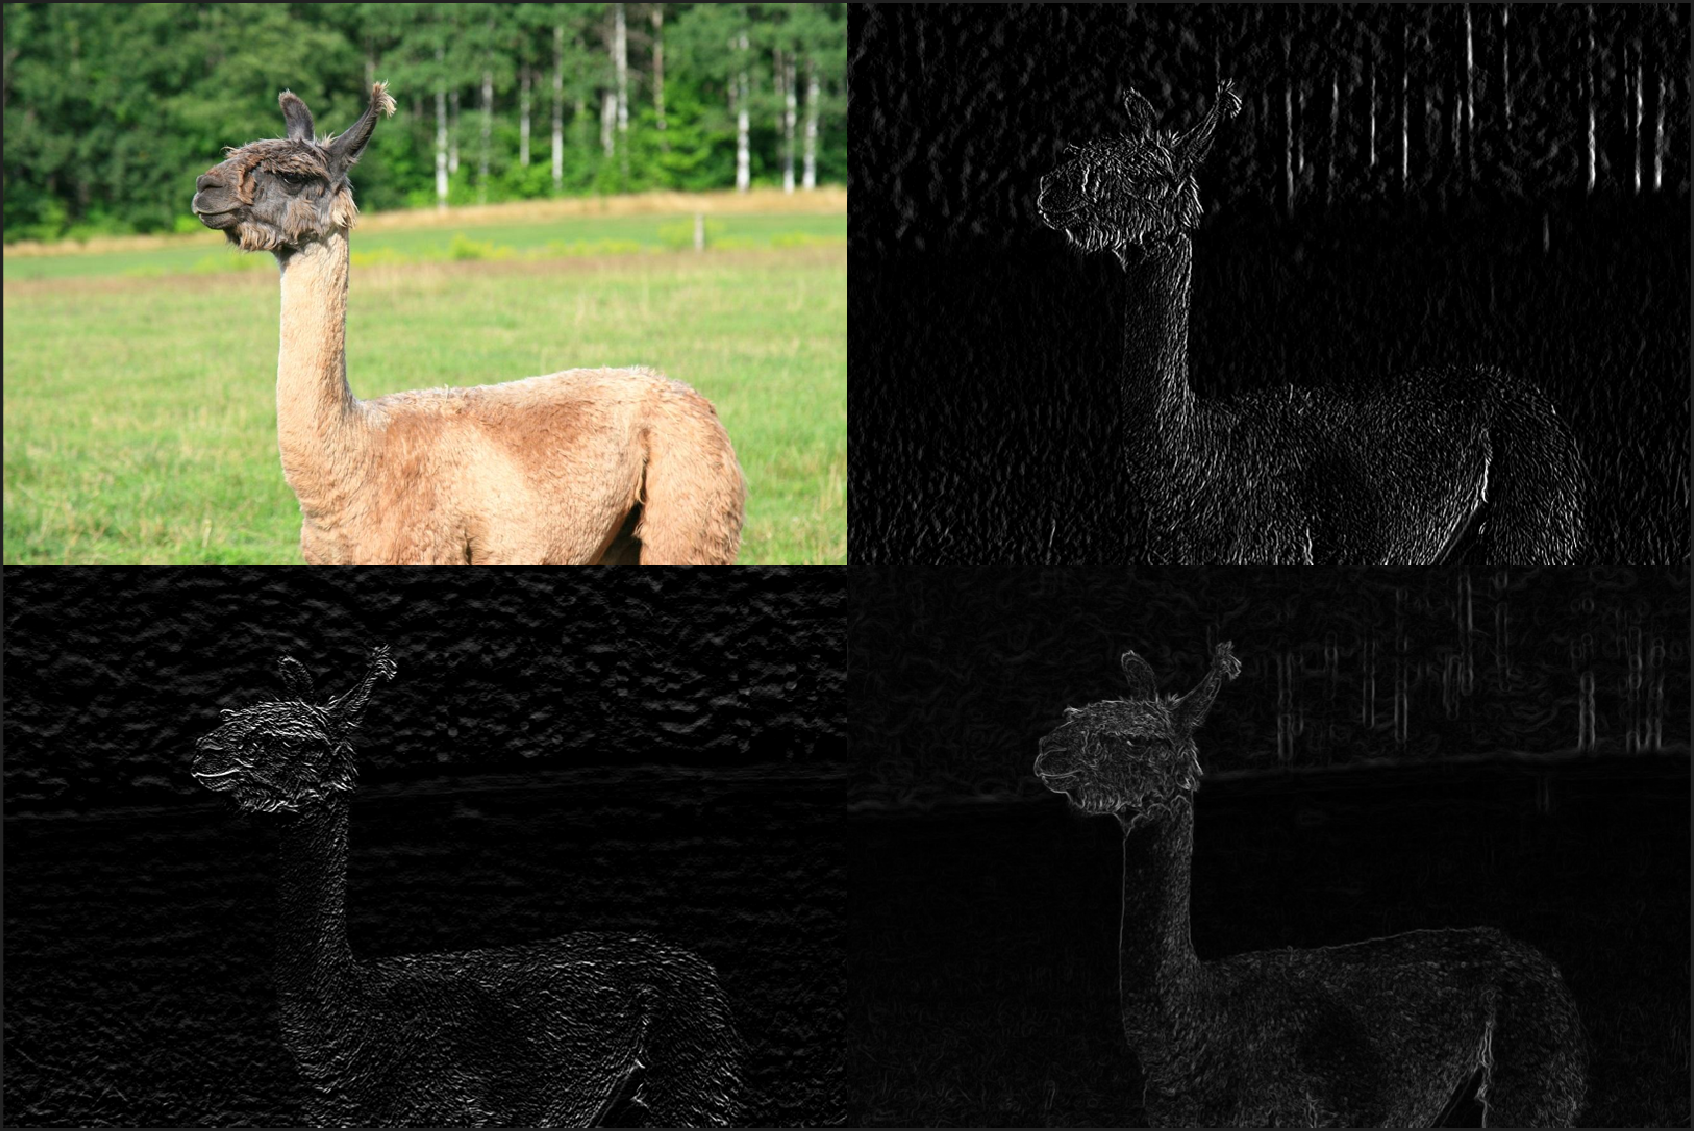
\includegraphics[scale = .4]{ejemplo_sobel}
			\caption{Detección de bordes aplicando los kernel Sobel}
			\label{fig:sobel}
		\end{figure}
		
		A continuación se va a calcular la convolución de la matriz del ejemplo anterior con $G_u$. Para verificar los cálculos, de nuevo se aplica la función \texttt{convn} de MATLAB. Al realizar los cálculos a mano tal y como se ha mostrado en el ejemplo anterior, se obtiene como resultado la matriz $A$, mientras que MATLAB devuelve la matriz $B$, esta vez los resultados no concuerdan. ¿Qué acaba de suceder? ¿Está mal codificada la función de MATLAB? ¿Está mal realizado el ejemplo?
		
		\begin{align*} A &= 
			\begin{pmatrix}
				4 & 4 & 4\\
				-4 & -4 & -4\\
				-4 & -4 & -4
			\end{pmatrix}&
			B &= \begin{pmatrix}
				-4 & -4 & -4\\
				4 & 4 & 4\\
				4 & 4 & 4
				\end{pmatrix}
		\end{align*}
		
		La respuesta a estas preguntas se podría resumir en que se ha realizado una ``pequeña trampa'' a la hora de explicar cómo calcular la convolución manualmente en el ejemplo, ya que no se ha aplicado correctamente la definición dada. ¿Qué sentido tiene hacer esto? En visión artificial y tratamiento de imágenes, muchos autores y librerías llaman convolución a la operación que se ha mostrado en el primer ejemplo, cuando en realidad no lo es y trae lugar a confusión. Dicha operación se llama correlación cruzada, denotada por $(\star)$, y que es muy similar a la convolución, pues su principal diferencia es que en la convolución ``real'', el kernel se rota 180 grados antes de calcular la convolución ``falsa'' o correlación cruzada, es decir, $X \ast Y = X \star (R_{180} \cdot Y)$, donde $R_{180}$ es la matriz de rotación de 180 grados. En el primer ejemplo se ha utilizado de manera intencionada la matriz $I_3$ para ver los casos que traen lugar a confusión, pues $I_3 \cdot R_{180} = I_3$. La correlación cruzada de dos imágenes (matrices) se define de la siguiente manera\cite{Goodfellow-et-al-2016}. 
		
		$$
		(f \star g)(u, v) = \sum_{i=-k}^{k}\sum_{j=-k}^{k} g(i, j)f(u + i, v + j)
		$$
		
		Esta operación sí es con la que realmente se aplican los filtros a las imágenes y con la que se trabaja en general en el campo de la visión artificial. Es importante ver que ahora, al contrario que con la convolución, $f \star g \neq g \star f$. Algunas librerías de visión artificial tratan a la correlación cruzada como convolución debido al frecuente uso que tiene una sobre la otra y la forma similar que tienen de calcularse. Un ejemplo es OpenCV para Python y C++ en la documentación de su función \texttt{filter2D}, donde se comenta que aplica una convolución cuando realmente aplica la correlación cruzada\cite{OpenCVFiltering}. Finalmente, como se verá en próximos capítulos, las famosas redes neuronales convolucionales, no aplican convoluciones sino correlaciones cruzadas. 
	\paginavacia
	\chapter{Aprendizaje automático y profundo}

	\section{Perceptrón}
	
		Ya en el año 1958, el psicólogo Frank Rosenblatt propuso un modelo llamado perceptrón el cual estaba basado en el comportamiento y funcionamiento de las neuronas de un humano, y que podía aprender ponderando cada coeficiente de entrada a la neurona\cite{historiaIA}. Hoy en día, tal y como se mostrará en esta sección, el perceptrón es la unidad fundamental de muchos modelos de \textit{machine learing} y \textit{deep learning}. \\
		
		Como se verá durante esta sección, este modelo ayuda a solucionar problemas de clasificación supervisada. Se dispone de una serie de valores de entrada $x_1, x_2, \hdots, x_n$ y se tiene una serie de valores de salida $y_1, y_2, \hdots, y_m$ que representan a qué clase pertenece la entrada ($2^m$ clases posibles). Esto se consigue mediante la ayuda de sus parámetros, que son una serie de pesos $w_1, w_2, \hdots, w_n$ y un sesgo o \textit{bias} $b$; y sus hiperparámetros, entre los que se encuentra una función $f$ de activación. 
		
		\begin{figure}[!h]
			\centering
			\begin{tikzpicture}
				\foreach \i in {1, 2}
					\pgfmathsetmacro{\resta}{int(\i - 1)}
					\node[circle, draw, fill=gray!20] (x-\i) at (0, -1 * \resta - \resta) {$x_{\i}$};
				\node (dots) at (0, -4) {$\vdots$};
				\node[circle, draw, fill=gray!20] (x-3) at (0, -6) {$x_{n}$};
				\node[circle, draw, fill=gray!20] (n) at (5,-3) {$n_1$};
				\node[circle, draw, fill=gray!20] (a) at (7,-3) {$a_1$};
				\node[circle, draw, fill=gray!20] (b) [below = of n] {$b_1$};
				\node[circle, draw, fill=gray!20] (y) [right = of a] {$y_1$};
				
				\foreach \i in {1, 2}
					\draw[-] (x-\i) -- (n) node [midway, above, sloped] {$w_{\i}$};
				\draw[-] (x-3) -- (n) node [midway, below, sloped] {$w_n$};
				\draw[-] (n) -- (a);
				\draw[-] (a) -- (y);
				\draw[-] (b) -- (n) node [midway, right] {$1$};
			\end{tikzpicture}
			\caption{Arquitectura de un perceptrón}
			\label{fig:perceptron}
		\end{figure}
		
		En la \Cref{fig:perceptron} se muestra la arquitectura del caso más simple de un perceptrón. Se tienen $n$ entradas y una única salida. La primera parte del diagrama representa que tal y como decía Rosenblatt, cada valor de entrada debe multiplicarse por un cierto peso, de tal forma que si se representa esto en función de sus valores en un instante $k$, lo que se computa en el nodo $n_1$ es la siguiente operación. 
		
		$$
		n_1(k) = b_1(k) + \sum_{i=1}^n x_i(k)w_i(k)
		$$
		
		Una vez se ha realizado este cálculo, el valor pasa por una función de activación en el nodo $a_1$, pues esta arquitectura es común utilizarla para clasificar una entrada y es muy útil obtener una salida binaria donde se active únicamente la salida que represente la clase a la que pertenece la entrada dada. Aunque existen diferentes funciones de activación para las neuronas, al trabajar con un perceptrón, la función de activación por excelencia es la función escalón de Heaviside, donde $\mathcal{U}: \mathbb{R} \longrightarrow \{0, 1\}$ y su expresión analítica es
		
		$$
		\mathcal{U}(x) = \left\{\begin{array}{ccc}
			0 & \text{si} & x < 0\\
			1 & \text{si} & x \geq 0
		\end{array}
		\right..
		$$
		
		Combinando ambas expresiones, se puede resumir en que la salida del perceptrón es equivalente a la siguiente ecuación: 
		
		$$
		y_1(k) = \left\{\begin{array}{ccc}
			0 & \text{si} & b_1(k) + \displaystyle\sum_{i=1}^n x_i(k)w_i(k) < 0\\
			1 & \text{si} & b_1(k) + \displaystyle\sum_{i=1}^n x_i(k)w_i(k) \geq 0
		\end{array}
		\right.
		$$
		
		Para dar un ejemplo claro de cómo funciona el perceptrón, se pueden tomar una serie de observaciones que tengan dos valores de entrada y uno de salida. Además, se supondrá que existen dos clases. Esto a fin de cuentas es asignar un valor de 0 o 1 a cada punto de $\mathbb{R}^2$ tal y como se describe en la \Cref{fig:labeled_data}. 
		
		\begin{figure}[!h]
			\centering
			\begin{tikzpicture}
				\begin{axis}[ymin = -2.5, ymax = 2.5, xmax = 2.5, xmin = -2.5, xticklabel = \empty, yticklabel = \empty, minor tick num = 1, axis lines = middle, xlabel = $x$, ylabel = $y$]
					\addplot[only marks, mark = *] coordinates {(1, 2)};
					\addplot[only marks, mark = triangle*] coordinates {(-1, 2) (0, -1)};
				\end{axis}
			\end{tikzpicture}
			\caption{Puntos etiquetados en $\mathbb{R}^2$}
			\label{fig:labeled_data}
		\end{figure}
		
		Una solución rápida sería trazar una recta $r: ax + by + c = 0$ que separe $\mathbb{R}^2$ en dos regiones, de forma que todo punto que pertenezca a una región pertenece entonces a una misma clase, tal y como se observa en la \Cref{fig:separated_label_data}. Esta recta suele llamarse \textit{decision boundary} o frontera de decisión. El problema entonces es hallar la recta $r$, pero se cumple que para este ejemplo es de la forma $w_1 x + w_2 y + b = 0$, siendo el problema encontrar los parámetros adecuados del modelo. La idea puede extrapolarse a diferente tamaño de entrada tomando un hiperplano de la forma $\textbf{w}^t \textbf{x} + b = 0$. \\
		
		Las preguntas a resolver ahora son, ¿existen siempre dichos parámetros? ¿Cómo pueden hallarse? El propio Minsky se hizo estas preguntas en \cite{perceptrons} y se dio cuenta de que dichos parámetros sí pueden hallarse en un número finito de pasos, siempre y cuando los puntos sean linealmente separables. Un ejemplo que no es linealmente separable es el de la función XOR tal y como se muestra en la \Cref{table:xor,fig:xor}, pues no existe una recta $r$ que separe $\mathbb{R}^2$ en dos regiones de tal forma que cada región contenga puntos de una única clase, sería necesaria una frontera de decisión no lineal. 
		
		\begin{figure}
			\centering
			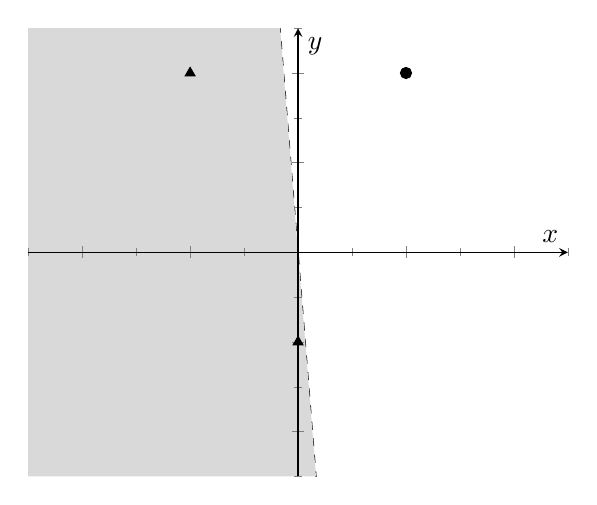
\begin{tikzpicture}
				\begin{axis}[ymin = -2.5, ymax = 2.5, xmax = 2.5, xmin = -2.5, xticklabel = \empty, yticklabel = \empty, minor tick num = 1, axis lines = middle, xlabel = $x$, ylabel = $y$, axis on top]
					\addplot[only marks, mark = *] coordinates {(1, 2)};
					\addplot[only marks, mark = triangle*] coordinates {(-1, 2) (0, -1)};
					\addplot[domain = -3:3, samples = 2, dashed] {-15*x};
					\draw[fill = gray!30, draw = none] (axis cs:-2.5, -2.5) -- (axis cs:-2.5, 2.5) -- (axis cs: -1/6, 2.5) -- (axis cs:1/6, -2.5);
				\end{axis}
			\end{tikzpicture}
			\caption{Puntos separados en $\mathbb{R}^2$}
			\label{fig:separated_label_data}
		\end{figure}
		
		\begin{table}[H]
			\centering
			\begin{tabular}{|c|c|c|}\hline
				$x$ & $y$ & $x \oplus y$\\\hline
				0 & 0 & 0\\\hline
				0 & 1 & 1\\\hline
				1 & 0 & 1\\\hline
				1 & 1 & 0\\\hline
			\end{tabular}
			\caption{Función XOR}
			\label{table:xor}
		\end{table}
		
		\begin{figure}
			\centering
			\begin{tikzpicture}
				\begin{axis}[ymin = -.5, ymax = 2.5, xmax = 2.5, xmin = -.5, xticklabel = \empty, yticklabel = \empty, minor tick num = 1, axis lines = middle, xlabel = $x$, ylabel = $y$]
					\addplot[only marks, mark = *] coordinates {(0, 0) (1, 1)};
					\addplot[only marks, mark = triangle*] coordinates {(0, 1) (1, 0)};
				\end{axis}
			\end{tikzpicture}
			\caption{Valores de $x \oplus y$ en  $\mathbb{R}^2$}
			\label{fig:xor}
		\end{figure}
		
		En cuanto a la pregunta de cómo hallar los parámetros, se consideran las siguientes ecuaciones\cite{nndesign}, donde $\textbf{w}$ es el vector de pesos, $t$ el valor esperado, y $a$ la salida del perceptrón y se aplica el \Cref{algo:perceptron} para obtener los parámetros óptimos. En dicho algoritmo se supondrá que existe una matriz $X$ de $n$ filas que contiene los diferentes $\textbf{x}$. 
		
		\begin{equation}
			\label{eq:perceptron}
			\begin{gathered}
				\textbf{w}(k+1) = \textbf{w}(k) + e(k)\textbf{x}(k)\\
				b(k+1) = b(k) + e(k)\\
				e(k) = t(k) - a(k)\\
				a(k) = \mathcal{U}(\textbf{w}^t(k)\textbf{x}(k))
			\end{gathered}
		\end{equation}
		
		
		\begin{algorithm}
			\SetProgSty{texttt}\DontPrintSemicolon
			
			\caption{Regla de aprendizaje del perceptrón}
			\label{algo:perceptron}
			
			\Datos{$X, \textbf{t}$}
			\Resultado{$\textbf{w}, b$}
			$b \gets 0$\\
			$\textbf{w} \gets$ \texttt{random}\\
			$k \gets 0$\\
			\Repetir{$\lnot$\texttt{acabar}}{
				\texttt{acabar} $\gets$ \texttt{true}\\
				\Para{$i \gets k$ \KwTo $k + n - 1$}{
					$e(i) \gets t(i) - a(i)$\\
					$\textbf{w}(i+1) \gets \textbf{w}(i) + e(i)\textbf{x}(i \pmod n)$\\
					$b(i+1) \gets b(i) + e(i)$\\
					\texttt{acabar} $\gets$ \texttt{acabar} $\land \, e(i) == 0$ 
				}
				$k \gets k + n - 1$
			}
		\end{algorithm}
		
		A cada una de las iteraciones que realiza el bucle exterior se les denomina épocas o \textit{epoch}, que consiste en realizar el proceso de entrenamiento sobre todo el conjunto de datos. En este caso se está suponiendo que no va a recibir casos que no sean linealmente separables, pero de lo contrario se puede añadir un contador \texttt{max\_epochs} y fijar un número máximo para no caer en un bucle infinito. No sería tarea fácil determinar dicho valor, pues aunque el algoritmo converge en los casos previamente explicados, no en todos lo hace de manera rápida. A continuación se muestra cómo obtener una solución para el caso de la \Cref{fig:labeled_data} aplicando el \Cref{algo:perceptron}. 
		
		$$
		X = \begin{pmatrix}
			1 & -1 & 0\\
			2 & 2 & -1
		\end{pmatrix} \,\,\, \textbf{t} = \begin{pmatrix}
		1 & 0 & 0
		\end{pmatrix} \,\,\, \textbf{w}(0) = \begin{pmatrix}
		1\\1 \end{pmatrix} \,\,\, b(0) = 0
		$$
		
		\begin{enumerate}[label = \textbf{\arabic*. }]
			\setcounter{enumi}{-1}
			\item \begin{itemize}
				\item $a(0) = \mathcal{U}(\textbf{w}^t(0)\textbf{x}(0)) = \mathcal{U}\left(\begin{pmatrix}1 & 1\end{pmatrix}\begin{pmatrix}
					1\\2 \end{pmatrix} + 0\right) = 1$
				\item $e(0) = t(0) - a(0) = 1 - 1 = 0$
				\item $\textbf{w}(1) = \textbf{w}(0)$
				\item $b(1) = b(0)$
			\end{itemize}
			
			\item \begin{itemize}
				\item $a(1) = \mathcal{U}(\textbf{w}^t(1)\textbf{x}(1)) = \mathcal{U}\left(\begin{pmatrix}1 & 1\end{pmatrix}\begin{pmatrix}
					-1\\2 \end{pmatrix} + 0\right) = 1$
				\item $e(1) = t(1) - a(1) = 0 - 1 = -1$
				\item $\textbf{w}(2) = \textbf{w}(1) + e(1)\textbf{x}(1) = \begin{pmatrix}1\\ 1\end{pmatrix} - \begin{pmatrix}-1\\2\end{pmatrix} = \begin{pmatrix}2\\ -1\end{pmatrix}$
				\item $b(2) = b(1) + e(1) = -1$
			\end{itemize}
			
			\item \begin{itemize}
				\item $a(2) = \mathcal{U}(\textbf{w}^t(2)\textbf{x}(2)) = \mathcal{U}\left(\begin{pmatrix}2 & -1\end{pmatrix}\begin{pmatrix}
					0\\-1 \end{pmatrix} -1\right) = 1$
				\item $e(2) = t(2) - a(2) = 0 - 1 = -1$
				\item $\textbf{w}(3) = \textbf{w}(2) + e(2)\textbf{x}(2) = \begin{pmatrix}2\\ -1\end{pmatrix} - \begin{pmatrix}0\\-1\end{pmatrix} = \begin{pmatrix}2\\ 0\end{pmatrix}$
				\item $b(3) = b(2) + e(2) = -2$
				\item $\texttt{acabar} = \texttt{true} \land \texttt{false} \land \texttt{false} = \texttt{false}$
			\end{itemize}
			
			\item \begin{itemize}
				\item $a(3) = \mathcal{U}(\textbf{w}^t(3)\textbf{x}(3\pmod{3})) = \mathcal{U}\left(\begin{pmatrix}2 & 0\end{pmatrix}\begin{pmatrix}
					1\\2 \end{pmatrix} -2\right) = 1$
				\item $e(3) = t(3) - a(3) = 1 - 1 = 0$
				\item $\textbf{w}(4) = \textbf{w}(3)$
				\item $b(4) = b(3)$
			\end{itemize}
			
			\item \begin{itemize}
				\item $a(4) = \mathcal{U}(\textbf{w}^t(4)\textbf{x}(4\pmod{3})) = \mathcal{U}\left(\begin{pmatrix}2 & 0\end{pmatrix}\begin{pmatrix}
					-1\\2 \end{pmatrix} -2\right) = 0$
				\item $e(4) = t(4) - a(4) = 0 - 0 = 0$
				\item $\textbf{w}(5) = \textbf{w}(4)$
				\item $b(5) = b(4)$
			\end{itemize}
			
			\item \begin{itemize}
				\item $a(5) = \mathcal{U}(\textbf{w}^t(5)\textbf{x}(5\pmod{3})) = \mathcal{U}\left(\begin{pmatrix}2 & 0\end{pmatrix}\begin{pmatrix}
					0\\-1 \end{pmatrix} -2\right) = 0$
				\item $e(5) = t(5) - a(5) = 0 - 0 = 0$
				\item $\textbf{w}(6) = \textbf{w}(5)$
				\item $b(6) = b(5)$
				\item $\texttt{acabar} = \texttt{true} \land \texttt{true} \land \texttt{true} = \texttt{true}$
			\end{itemize}
		\end{enumerate}
		
		La ejecución del algoritmo finaliza tras dos épocas, donde en la primera de ellas va ajustando los pesos y el sesgo de manera adecuada, y en la segunda verifica que todas las observaciones han sido clasificadas de manera correcta. La frontera de decisión obtenida es la recta $r: 2x - 2 = 0$, que es una recta vertical. Una observación a realizar es que $\textbf{x}(1) \in r$, por tanto ¿a qué clase pertenece? Esto depende de la función de activación empleada, al utilizar $\mathcal{U}$ la clasificación es correcta, pero al cambiarla por otra, podría no serlo y necesitaría de más épocas para realizar correctamente la clasificación. \\
		
		La última cuestión que queda por tratar respecto al perceptrón es el porqué se verifica que en el caso de que los puntos dados sean linealmente separables, en un número finito de pasos, el \Cref{algo:perceptron} terminará su ejecución y con el $\textbf{w}$ óptimo, tal y como se enunciaba en el \textbf{Teorema de Convergencia del Perceptrón}. A continuación se realiza su demostración basándose en la que se encuentra en \cite{nndesign} pero de forma más clara y simple. Para comenzar con la demostración será necesario definir una serie de elementos, comenzando por $\Omega(k)$ y $\textbf{z}(k)$. Se entiende que se están concatenando vectores, no definiendo ``vectores dentro de vectores''. 
		
		$$
		\Omega(k) = \begin{pmatrix}
			\textbf{w}(k)\\
			b(k)
		\end{pmatrix} \,\,\, \textbf{z}(k) = \begin{pmatrix}
		\textbf{x}(k)\\
		1
		\end{pmatrix}
		 \,\,\, \Omega(0) = \begin{pmatrix}
			0\\0\\\vdots\\0
		\end{pmatrix}
		$$
		
		Con estos elementos y el cálculo de $a(k)$ en la \Cref{eq:perceptron} es fácil ver que $n(k) = \Omega^t(k)\textbf{z}(k)$. Recordando los posibles valores de $t(k)$, se deseaba que si dicho valor era 1, entonces $n(k) \geq 0$; y en caso de que valiese 0 entonces se deseaba tener $n(k) < 0$, en resumen, que $t(k) - a(k) = 0$. Otra forma de ver esto es afirmar que en el caso en que $t(k) \neq a(k)$, entonces $\Omega(k)$ debe actualizarse de acuerdo a la \Cref{eq:perceptron}. De esta forma $\Omega(k + 1) = \Omega(k) + e(k)\textbf{z}(k)$. Ahora se considerará un vector $\Omega^*$ de forma que 
		$$
		\forall k \exists \Omega^* \,\, \mathcal{U}(\Omega^{*^t}\textbf{z}(k)) = t(k),
		$$
		es decir, $\Omega^*$ es el vector de pesos óptimo. Además, por comodidad se normalizarán todas las distancias del problema, de manera que $\|\Omega^{*}\| = 1$ y $\|\textbf{z}(k)\| \leq 1$. El último elemento a considerar será $\delta$, que será definido como
		$$
		\delta = \min\lbrace\Omega^{*^t}\textbf{z}(i)\rbrace, 
		$$
		tomando además que $\delta > 0$ pues otra manera de definirlo es la distancia al punto más cercano a la frontera de decisión óptima. Con estos elementos se puede comenzar la demostración. Como la regla de actualización es $\Omega(k + 1) = \Omega(k) + e(k)\textbf{z}(k)$, al vector de pesos en un determinado instante (clasificación fallida) se le suma o resta $\textbf{z}(k)$ y a priori no se sabe cuántas veces se va a repetir esto, por lo que la idea de la demostración será ver si la norma del vector de pesos tiene una cota superior e inferior, es decir, se para de sumar o restar otros vectores $\textbf{z}(i)$, de manera que el algoritmo terminaría. Para obtener esto basta con comparar el comportamiento de $\Omega^t(k) \Omega^*$ frente a $\Omega^t(k)\Omega(k)$ (es decir, $\|\Omega\|^2$). \\
		
		Con el primero de los términos, al tratar de corregir un error se verifica que
		
		$$
		\Omega^t(k+1)\Omega^* = (\Omega(k) + e(k)\textbf{z}(k))^t \Omega^* = \Omega^t(k)\Omega^* + e(k)\Omega^{*^t}\textbf{z}(k). 
		$$
		
		Además, por la manera en la que se ha definido $\delta$, el segundo sumando pertenece al intervalo $(-\infty, -\delta] \cup [\delta, \infty)$, pudiendo deducir la siguiente desigualdad, por lo que en una actualización el término sólo varía por lo menos en $\delta$ unidades.  
		
		\begin{equation}
			\label{eq:inf_delta}
			\Omega^t(k+1)\Omega^* \geq \Omega^t(k)\Omega^* + \delta
		\end{equation}
		
		De la misma manera que se ha analizado el comportamiento de $\Omega^t(k) \Omega^*$ se procede con la actualización de $\Omega^t(k)\Omega(k)$. 
		
		\begin{align*}
			\Omega^t(k+1)\Omega(k+1) &= (\Omega(k) + e(k)\textbf{z}(k))^t(\Omega(k) + e(k)\textbf{z}(k))\\
			&= \Omega^2(k) + (e(k)\textbf{z}(k))^2 + 2e(k)\Omega^t(k)\textbf{z}(k)\\
			&= \Omega^t(k)\Omega(k) + e^2(k)\textbf{z}^t(k)\textbf{z}(k) + 2e(k)\Omega^t(k)\textbf{z}(k)\\
			&= \Omega^t(k)\Omega(k) + e^2(k)\textbf{z}^t(k)\textbf{z}(k) + 2e(k)n(k)
		\end{align*}
		
		En el segundo sumando se tiene que siempre será menor o igual que 1, pues por definición $0 \leq \textbf{z}^t(k)\textbf{z}(k) = \|\textbf{z}(k)\|^2 \leq 1$. Además, el tercer sumando siempre será cero o negativo, pues en todos los casos posibles en los que $e(k) \neq 0$ se cumple que $e(k)n(k) < 0$: 
		
		\begin{itemize}
			\item Si $t(k) = 1 \land n(k) < 0$, entonces $a(k) = 0 \land e(k) > 0$
			\item Si $t(k) = 0 \land n(k) \geq 0$, entonces $a(k) = 1 \land e(k) < 0$
		\end{itemize}
		
		De esta situación se puede deducir la siguiente desigualdad, por lo que en una actualización el término sólo varía en como máximo una unidad.   
		
		\begin{equation}
			\label{eq:sup_delta}
			\Omega^t(k+1)\Omega(k+1) \leq \Omega^t(k)\Omega(k) + 1
		\end{equation}
		
		Una vez se ha observado cómo varían estos términos al actualizarlos, se puede observar qué pasaría con ellos al hacer $m$ actualizaciones. Con el resultado obtenido en las \Cref{eq:inf_delta,eq:sup_delta} se pueden deducir las desigualdades $\delta m \leq \Omega^t(m)\Omega^*$ y $\Omega^t(m)\Omega(m) \leq m$. \\
		
		Ahora al aplicar la desigualdad de Cauchy--Schwarz\footnote{Esta desigualdad afirma que $\|\textbf{u}\textbf{v}\| \leq \|\textbf{u}\|\|\textbf{v}\|$. }, el valor de $\|\Omega^*\|$, y la propiedad transitiva, se obtiene una cota superior y otra inferior (ambas recuadradas) para $\|\Omega^t(m)\|$, lo que demuestra que el número de actualizaciones es finito y que por tanto el algoritmo converge. 
		
		\begin{align*}
			\boxed{\delta m} &\leq \Omega^t(m)\Omega^* = \|\Omega^t(m)\Omega^*\|\\
			&\leq \|\Omega^t(m)\| \|\Omega^*\| = \|\Omega^t(m)\| = \sqrt{\Omega^t(m)\Omega(m)}\\
			& \leq \boxed{\sqrt{m}} 
		\end{align*}
		
		$$
		\pushQED{\qed} 
		\delta m \leq \|\Omega(m)\| \leq \sqrt{m} \,\,\, \Longrightarrow \,\,\, m \leq \frac{1}{\delta^2}\qedhere
		\popQED
		$$ 
		
		Esta última desigualdad muestra cómo existe una relación entre el número de iteraciones del algoritmo y la distancia de los datos de entrenamiento a la frontera de decisión óptima (depende únicamente de esto). Cuanto más cerca estén, mayor será el número de iteraciones necesarias. 
		
	\section{Redes neuronales artificiales}
	
		El descubrimiento del perceptrón junto con el teorema que garantizaba que cualquier conjunto de puntos linealmente separable podría ser aprendido mediante este, supuso un gran avance en la IA al igual que una gran desilusión por parte de muchos al no poder aprender una función tan simple como la XOR. Esto causó el llamado el primer invierno de la IA, que finalizó con la llegada de las redes neuronales multicapa y el algoritmo de la retroprogragación. \\
		
		En 1989, George Cybenko enunció y consiguió demostrar el \textbf{Teorema de Aproximación Universal}\cite{teoremaAproximacion}. Este afirma que dada una red neuronal con una capa de entrada, una capa oculta con suficientes neuronas, y una capa de salida; es un aproximador universal de funciones. Es decir, si existe una relación entre dos variables $\textbf{x}$ e $\textbf{y}$, entonces una red neuronal con la arquitectura mencionada y el entrenamiento adecuado, encontrará dicha relación y podrá comportarse como una función $f$ tal que $\textbf{y} = f(\textbf{x})$. Este se considera un gran resultado, pues consigue acabar con las limitaciones del perceptrón que habían generado un decaimiento por el interés en la IA. 
		
		\begin{figure}[!h]
			\centering
			\begin{tikzpicture}
				\node[circle, draw, fill=gray!20] (x-1) {$x_{1}$};
				\foreach \i in {2,3}{
					\pgfmathtruncatemacro{\resta}{\i - 1}
					\node[circle, draw, fill=gray!20, below = of x-\resta] (x-\i) {$x_{\i}$};
				}
				\node (dots) [below = of x-3] {$\vdots$};
				\foreach \i in {1,2,3}{
					\node[circle, draw, fill=gray!20, right = 2cm of x-\i] (a-\i) {$a^{(1)}_{\i}$};
				}
				\node (dots2) [below = of a-3] {$\vdots$};
				\node (a-4) [circle, draw, fill=gray!20, below = of dots2] {$a^{(1)}_i$};
				\foreach \i in {1,2,3}{
					\node[circle, draw, fill=gray!20, right = 2cm of a-\i] (A-\i) {$a^{(M)}_{\i}$};
				}
				\node (dots3) [below = of A-3] {$\vdots$};
				\node (x-4) [circle, draw, fill=gray!20, left = 2cm of a-4] {$x_n$};
				\node (A-4) [circle, draw, fill=gray!20, below = of dots3] {$a^{(M)}_j$};
				\foreach \i in {1,2,3,4}{
					\node [left = .6cm of A-\i] {$\cdots$};
					\foreach \j in {1,2,3,4}{
						\draw[-] (x-\i) -- (a-\j);
					}
				}
				\foreach \i in {1,2,3}{
					\node (y-\i) [circle, draw, fill=gray!20, right =  of A-\i] {$y_{\i}$};
					\draw[-] (A-\i) -- (y-\i);
				}
				\node (y-4) [circle, draw, fill=gray!20, right =  of A-4] {$y_{j}$};
				\draw[-] (A-4) -- (y-4);
				\node (dots4) [right = 1.6cm of dots3] {$\vdots$};
			\end{tikzpicture}
			\caption{Arquitectura de una red neuronal multicapa}
			\label{fig:rna}
		\end{figure}
		
		En la \Cref{fig:rna} se muestra un diagrama que resume la arquitectura de una red neuronal multicapa. Todas las salidas de una capa están conectadas con todas las entradas de la siguiente con un peso y un \textit{bias}. En el diagrama de la \Cref{fig:rna_completa} se puede observar esto en mayor detalle. Estas pueden ser utilizadas en problemas de clasificación o regresión supervisada, pero en una primera aproximación se supondrá que se está resolviendo un problema de regresión. \\
		
		\begin{figure}
			\centering
			\resizebox{\textwidth}{!}{
				\begin{tikzpicture}
					\node[circle, draw, fill=gray!20] at (4, 0) (n-1) {$n^{(1)}_{1}$};
					\node[circle, draw, fill=gray!20, below= .5cm of n-1] (b-1) {$b^{(1)}_{1}$};
					\foreach \i in {2,3}{
						\pgfmathtruncatemacro{\resta}{\i - 1}
						\node[circle, draw, fill=gray!20, below= 2 cm of b-\resta] (n-\i) {$n^{(1)}_{\i}$};
						\node[circle, draw, fill=gray!20, below= .5cm of n-\i] (b-\i) {$b^{(1)}_{\i}$};
					}
					\node[circle, draw, fill=gray!20, below left = 2 cm and 7 cm of n-1] (x-1) {$x_{1}$};
					\foreach \i in {2,3}{
						\pgfmathtruncatemacro{\resta}{\i - 1}
						\node[circle, draw, fill=gray!20, below= 2cm of x-\resta] (x-\i) {$x_{\i}$};
					}
					\node (dots) [below = .5cm of x-3] {$\vdots$};
					\node[circle, draw, fill=gray!20, below = .5cm of dots] (x-n) {$x_{n}$};
					\node (dots2) [below = .5cm of b-3] {$\vdots$};
					\node[circle, draw, fill=gray!20, below= .5cm of dots2] (n-n) {$n^{(1)}_{i}$};
					\node[circle, draw, fill=gray!20, below= .5cm of n-n] (b-n) {$b^{(1)}_{i}$};
					\foreach \i in {1,2,3}{
						\draw[-] (n-\i) -- (b-\i) node [midway, right] {$1$};
					}
					\draw[-] (b-n) -- (n-n) node [midway, right] {$1$};
					\foreach \i in {1,2,3}{
						\foreach \j in {1,2,3}{
							\pgfmathtruncatemacro{\condicion}{ifthenelse(Mod(\i, 2)==0,1,0)}
							\ifnum\condicion=1
							\draw[-] (x-\i) -- (n-\j) node [near start, above, sloped] {$w^{(1)}_{\j\i}$};
							\else
							\draw[-] (x-\i) -- (n-\j) node [near end, above, sloped] {$w^{(1)}_{\j\i}$};
							\fi
						}
					}
					\foreach \i in {1,2,3}{
						\draw[-] (x-n) -- (n-\i) node [near start, above, sloped] {$w^{(1)}_{\i n}$};
						\draw[-] (x-\i) -- (n-n) node [near end, below, sloped] {$w^{(1)}_{i\i}$};
					}
					\draw[-] (x-n) -- (n-n) node [midway, below, sloped] {$w^{(1)}_{in}$};
					\foreach \i in {1,2,3}{
						\node[circle, draw, fill=gray!20, right = 1cm of n-\i] (a-\i) {$a^{(1)}_{\i}$};
					}
					\node[circle, draw, fill=gray!20, right = 1cm of n-n] (a-n) {$a^{(1)}_{i}$};
					\foreach \i in {1,2,3}{
						\draw[-] (n-\i) -- (a-\i);
					}
					\draw[-] (n-n) -- (a-n);
					\foreach \i in {1,2,3}{
						\node [right = .7cm of a-\i] {$\cdots$};
						\node[circle, draw, fill=gray!20, right = 2cm of a-\i] (N-\i) {$n^{(M)}_{\i}$};
					}
					\node[circle, draw, fill=gray!20, right = 2cm of a-n] (N-4) {$n^{(M)}_{j}$};
					\node [right = .7cm of a-n] {$\cdots$};
					\foreach \i in {1,2,3}{
						\node[circle, draw, fill=gray!20, right = 1cm of N-\i] (A-\i) {$a^{(M)}_{\i}$};
					}
					\node[circle, draw, fill=gray!20, right = 1cm of N-4] (A-4) {$a^{(M)}_{j}$};
					\foreach \i in {1,2,3,4}{
						\draw[-] (N-\i) -- (A-\i);
					}
					\foreach \i in {1,2,3}{
						\node[circle, draw, fill=gray!20, below= .5cm of N-\i] (B-\i) {$b^{(M)}_{\i}$};
						\draw[-] (N-\i) -- (B-\i) node [midway, right] {$1$};
					}
					\node [below = .5cm of B-3] {$\vdots$};
					\node[circle, draw, fill=gray!20, below= .5cm of N-4] (B-4) {$b^{(M)}_{j}$};
					\draw[-] (N-4) -- (B-4) node [midway, right] {$1$};
					\foreach \i in {1,2,3}{
						\node[circle, draw, fill=gray!20, right = 22 cm of x-\i] (y-\i) {$y_{\i}$};
					}
					\node[circle, draw, fill=gray!20, right = 22 cm of x-n] (y-4) {$y_{j}$};
					\foreach \i in {1,2,3,4}{
						\draw[-] (A-\i) -- (y-\i);
					}
				\end{tikzpicture}
			}
			\caption{Red neuronal multicapa}
			\label{fig:rna_completa}
		\end{figure}
		
		Al igual que un perceptrón quedaba representado mediante un vector $\textbf{w}$ de pesos y un valor de sesgo $b$, para representar una red neuronal multicapa se hace mediante las matrices $W^{(m)}$ y los vectores $\textbf{b}^{(m)}$ y $\textbf{f}^{(m)}$, que contienen los pesos, los sesgos, y las funciones de activación. La notación para los sesgos es $b_i^{(m)}$, que representa el sesgo de la entrada $i-$ésima de la capa $m$. De igual manera $f_i^{(m)}$ representa la función de activación la neuona $i-$ésima de la capa $m$. Para los pesos, $w_{ij}^{(m)}$ denota el peso que une la salida $j$ con la entrada $i$ de la capa $m$. Para las capas, $1 \leq m < M$. En ningún momento un exponente entre paréntesis representa una potencia, en dicho caso aparecerá sin paréntesis para distinguirlo. Siguiendo los mismos pasos que con el perceptrón, la primera pregunta será cómo calcular la salida de una red neuronal. La salida de una capa se calcula con la \Cref{eq:prop}, teniendo en cuenta que $\textbf{x}^{(m)} = \textbf{y}^{(m-1)}$, por lo que para calcular la salida de la red no hay más que aplicar dicha ecuación hasta llegar a la última capa. 
		
		\begin{equation}
			\label{eq:prop}
			\begin{gathered}
				\textbf{a}^{(m)}(k) = \textbf{f}^{(m)}\left(W^{(m)}(k)\textbf{x}^{(m)}(k) + \textbf{b}^{(m)}(k)\right)\\
				\begin{pmatrix}
					a_1^{(m)}(k)\\a_2^{(m)}(k)\\\vdots\\a_j^{(m)}(k)
				\end{pmatrix} = \textbf{f}^{(m)}\left(
				\begin{pmatrix}
					w_{11}^{(m)}(k) & w_{12}^{(m)}(k) & \cdots & w_{1i}^{(m)}(k)\\
					w_{21}^{(m)}(k) & w_{22}^{(m)}(k) & \cdots & w_{2i}^{(m)}(k)\\
					\vdots & \vdots & \ddots & \vdots\\
					w_{j1}^{(m)}(k) & w_{j2}^{(m)}(k) & \cdots & w_{ji}^{(m)}(k)\\
				\end{pmatrix}
				\begin{pmatrix}
					x_1^{(m)}(k)\\x_2^{(m)}(k)\\\vdots\\x_i^{(m)}(k)
				\end{pmatrix} + 
				\begin{pmatrix}
					b_1^{(m)}(k)\\b_2^{(m)}(k)\\\vdots\\b_j^{(m)}(k)
				\end{pmatrix}\right)
			\end{gathered}
		\end{equation}
		
		A continuación, se puede plantear cuál es la ecuación del error para una red neuronal. Esta es simplemente cuestión de elección al igual que las funciones de activación. Al trabajar con redes neuronales para problemas de regresión, la función de error por excelencia es el error cuadrático, definido como
		$$
		L(k) = \sum(\textbf{t}(k) - \textbf{a}^{(M)}(k))^2, 
		$$
		aunque existen otras muchas, cada una adecuada a cada tipo de problema y modelo, como por ejemplo el error cuadrático medio, error absoluto, error absoluto medio, error logarítmico, error exponencial, entropía cruzada, etc\cite{funcionesError}.\\
		
		La pregunta ahora sería que, al igual que existía una ecuación para actualizar los parámetros del perceptrón ¿existe para una red neuronal? Para deducirla fácilmente, basta en pensar que $L$ es una función que depende de los parámetros de la red y que se quiere que su valor sea lo más pequeño posible para diferentes vectores de entrada, es decir, encontrar los valores de los parámetros que minimizan $L$. Esto es un problema clásico de cálculo que en el caso de una variable se resuelve igualando a cero la derivada de la función, y en el caso de varias, mediante la matriz Hessiana. Sin embargo, dichos métodos para una función de tantas variables y con expresiones complejas, no son muy eficientes. \\
		
		Esto se soluciona con ayuda de un algoritmo conocido como descenso por gradiente\cite{descenso}. Este algoritmo calcula de manera iterativa una aproximación de los mínimos de una función con ayuda del vector gradiente de una función. El vector gradiente de una función $f$ se define como 
		$$
		\nabla f(x_1, x_2, \hdots, x_n) = \left(\frac{\partial f}{\partial x_1}, \frac{\partial f}{\partial x_2}, \hdots, \frac{\partial f}{\partial x_n}\right), 
		$$
		e indica la dirección en la que la función crece más rápido, siendo la idea principal del algoritmo ir moviéndose en dirección contraria a este. 
		
		\begin{algorithm}
			\SetProgSty{texttt}\DontPrintSemicolon
			
			\caption{Descenso por gradiente}
			\label{algo:descenso}
			
			\Datos{$f, \alpha, k$}
			\Resultado{$\textbf{x}(k)$}
			$\textbf{x}(0) \gets$\texttt{ random}\\
			\Para{$i \gets 1$ \KwTo $k$}{
				$\textbf{x}(i + 1) = \textbf{x}(i) - \alpha\nabla f(\textbf{x}(i))$
			}
		\end{algorithm}
		
		Como se observa en el \Cref{algo:descenso}, se comienza en un punto aleatorio, lo que puede variar la calidad de la solución dependiendo de la ejecución, y además se introduce un término $\alpha$ llamado \textbf{tasa de aprendizaje}. Pueden existir casos en los que la magnitud del gradiente sea muy grande, lo que resulta en desplazamientos bruscos y una convergencia más lenta, tal y como se refleja en la \Cref{fig:descenso}. Si se hubiese fijado un valor máximo de $k = 25$, en los casos de las \Cref{fig:descenso_grande,fig:descenso_peq}, no se hubiese llegado a una buena aproximación del mínimo por haber elegido un $\alpha$ inadecuado. 
		
		\begin{figure}[H]
			\centering
			\begin{subfigure}{.3\textwidth}
				\centering
				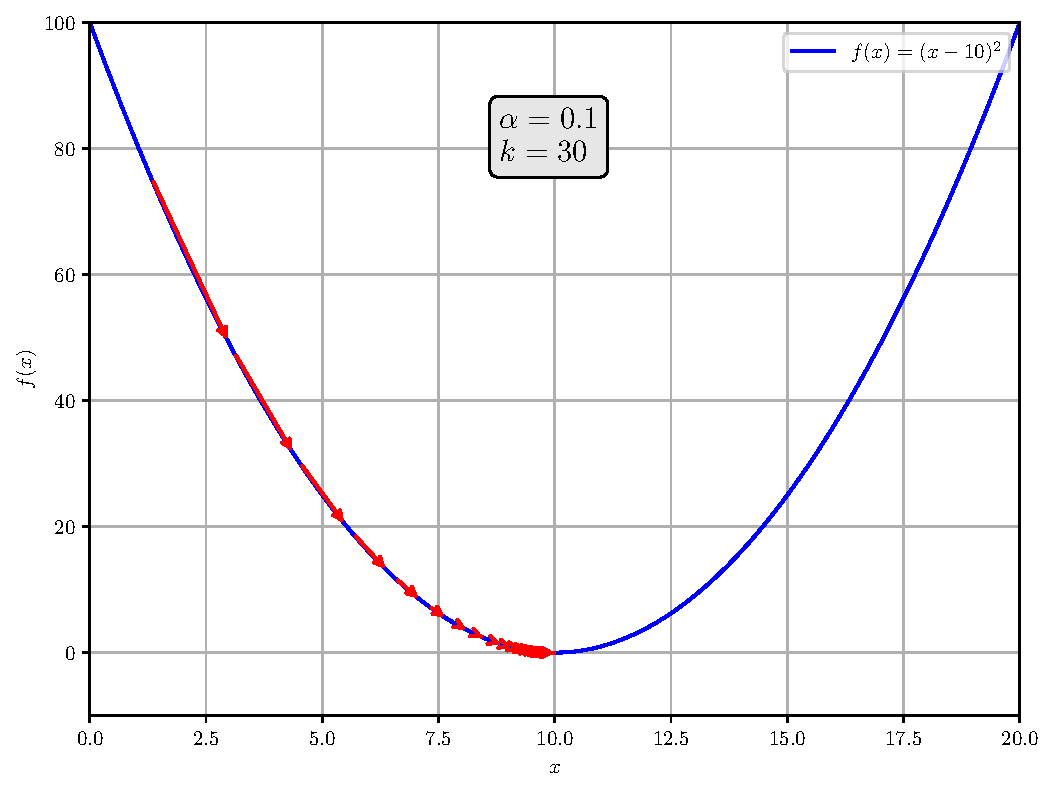
\includegraphics[width = \linewidth]{descenso}
				\caption{$\alpha$ adecuada}
			\end{subfigure}
			\begin{subfigure}{.3\textwidth}
				\centering
				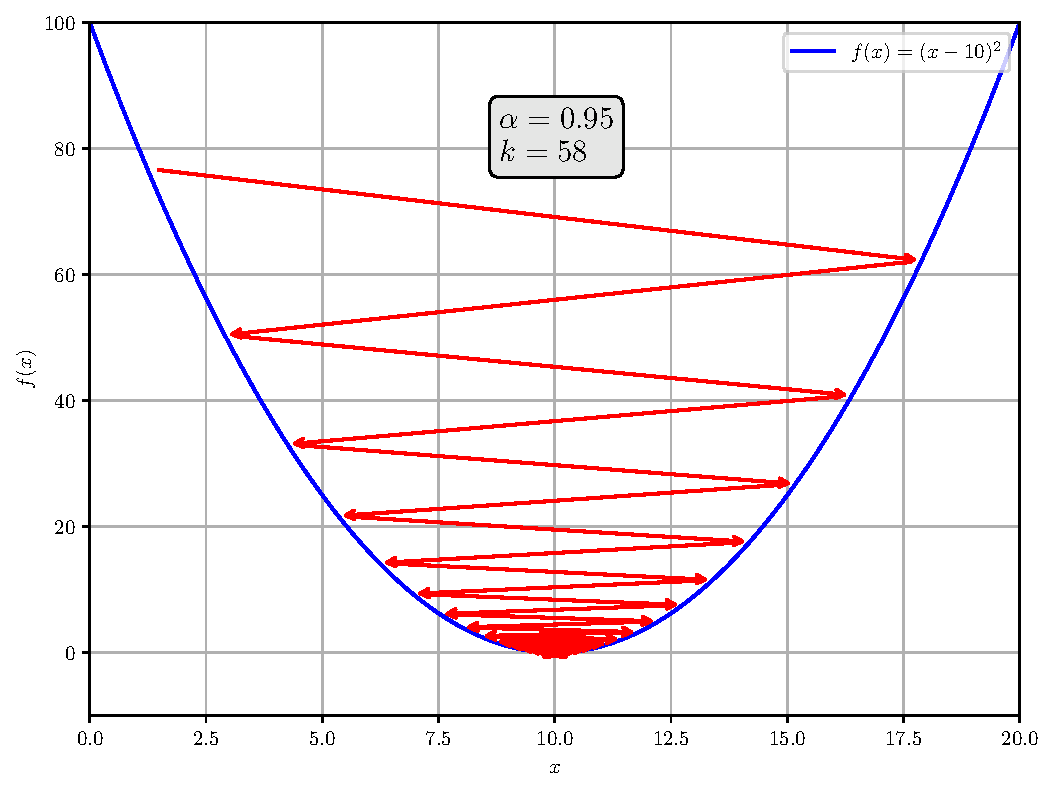
\includegraphics[width = \linewidth]{descenso2}
				\caption{$\alpha$ demasiado grande}
				\label{fig:descenso_grande}
			\end{subfigure}
			\begin{subfigure}{.3\textwidth}
				\centering
				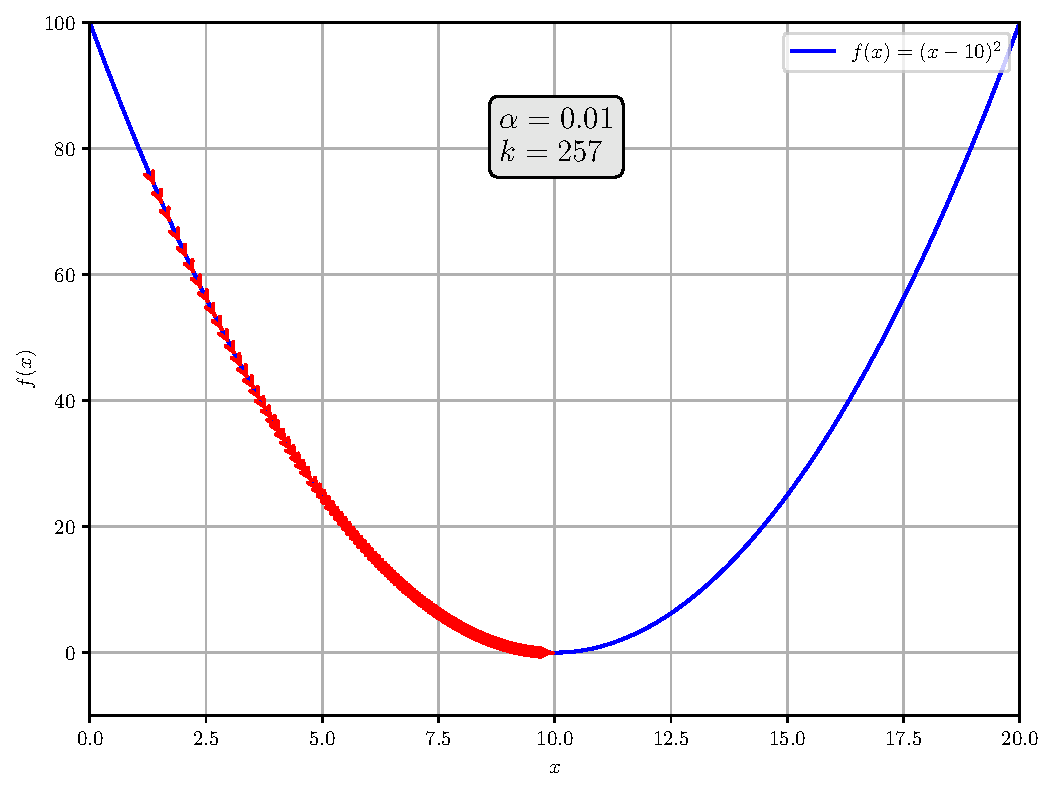
\includegraphics[width = \linewidth]{descenso3}
				\caption{$\alpha$ demasiado pequeña}
				\label{fig:descenso_peq}
			\end{subfigure}
			\caption{Descenso por gradiente}
			\label{fig:descenso}
		\end{figure}
		
		Con esta idea de la función de error y el descenso por gradiente, aparece el famoso algoritmo de la retropropagación o \textit{backpropagation}. Es muy similar al algoritmo de aprendizaje del perceptrón pero adaptado a la estructura de una red neuronal. El primer paso consiste en dada una entrada, calcular la salida de la red con ayuda de la \Cref{eq:prop}. El segundo paso es calcular el error $L(k)$. Esta función depende de todos los pesos y sesgos de la red, por lo que el tercer paso será modificar estos de acuerdo a $\nabla L$ y repetir el procedimiento para el resto de observaciones. Se realizan tantas épocas como sean necesarias. \\
		
		El problema que queda por resolver es cómo calcular todos los elementos de $\nabla L$, pues por ejemplo es fácil calcular $\frac{\partial L}{\partial a_i^{(M)}}$, pero no parece tan obvio calcular $\frac{\partial L}{\partial w_{ij}^{(m)}}$, pues hay que retroceder $M-m$ capas, y habrá muchos valores que dependan de ese peso. La solución a esto es la regla de la cadena. 
		
		$$
		\frac{\partial f}{\partial x} = \sum_{i=1}^n \frac{\partial f}{\partial u_{i1}}\frac{\partial u_{im}}{\partial x}\prod_{j=1}^{m-1}\frac{\partial u_{ij}}{\partial u_{ij+1}}
		$$
		
		Con ayuda de esta regla se pueden calcular fácilmente los términos no triviales del gradiente, propagando el error hacia atrás por la red hasta llegar al parámetro deseado mediante las sensibilidades $\left(\delta_i^{(s)}\right)$\cite{nndesign}. De aquí se intuye el porqué del nombre del algoritmo. De manera informal, lo que hace el algoritmo es castigar a cada neurona de manera proporcional a su participación en el error final. 
		
		$$
		\begin{gathered}
			\frac{\partial L}{\partial b_{i}^{(s)}} = \frac{\partial L}{\partial a_{i}^{(s)}} \frac{\partial a_{i}^{(s)}}{\partial n_{i}^{(s)}} \frac{\partial n_{i}^{(s)}}{\partial b_{i}^{(s)}} = \delta_i^{(s)}\\
			\frac{\partial L}{\partial w_{ij}^{(s)}} = \frac{\partial L}{\partial a_{i}^{(s)}} \frac{\partial a_{i}^{(s)}}{\partial n_{i}^{(s)}} \frac{\partial n_{i}^{(s)}}{\partial w_{ij}^{(s)}} = \delta_i^{(s)} \frac{\partial n_{i}^{(s)}}{\partial w_{ij}^{(s)}} = \delta_i^{(s)} a_j^{(s-1)}\\
			\delta_i^{(M)} = \frac{\partial L}{\partial a_{i}^{(M)}} \frac{\partial a_{i}^{(M)}}{\partial n_{i}^{(M)}} = -2a_{i}^{(M)} \frac{\partial a_{i}^{(M)}}{\partial n_{i}^{(M)}} = -2a_{i}^{(M)} \frac{\partial f_{i}^{(M)}}{\partial n_{i}^{(M)}}\\
			\delta_i^{(m)} = \frac{\partial L}{\partial n_i^{(m)}} = \sum_{l=1}^p\frac{\partial L}{\partial n_l^{(m+1)}}\frac{\partial n_l^{(m+1)}}{\partial n_i^{(m)}} = \sum_{l=1}^p \delta_l^{(m+1)} \frac{\partial n_l^{(m+1)}}{\partial n_i^{(m)}} = \sum_{l=1}^p \delta_l^{(m+1)} w_{li}^{(m+1)} \frac{\partial f_i^{(m)}}{\partial n_i^{(m)}}\\
			\text{con } 0 < m < M \text{ y } 0 < s \leq M
		\end{gathered}
		$$
		
		Estas ecuaciones pueden reescribirse de manera matricial para aligerar la notación, que combinándolas con las ideas explicadas referentes al \Cref{algo:descenso}, da lugar al \Cref{algo:backprop}, bastante similar al \Cref{algo:perceptron} pero adaptado a una red neuronal. \\
		
		\begin{algorithm}
			\SetProgSty{text}\DontPrintSemicolon
			
			\caption{Retropropagación (\textit{backpropagation})}
			\label{algo:backprop}
			
			\Datos{$\textbf{f}^{(s)}, \textbf{x}^{(1)}(k), \textbf{t}(k), \varepsilon$}
			\Resultado{$W^{(s)}, \textbf{b}^{(s)}$}
			
			\Para{$i \gets 1$ \KwTo $\varepsilon$}{
				\ParaCada{$\textbf{x}^{(1)}$}{
					\texttt{calcular} $\textbf{a}^{(M)}(k)$\\
					\texttt{calcular} $L(k)$ y $\nabla L(k)$\\
					$
					\begin{gathered}
						\delta^{(M)}(k) \gets -2 \frac{\partial \textbf{f}^{(M)}}{\partial \textbf{n}^{(M)}}(\textbf{t}(k) - \textbf{a}^{(M)}(k))\\
						\delta^{(m)}(k) \gets \frac{\partial \textbf{f}^{(M)}}{\partial \textbf{n}^{(M)}} W^{(m+1)^t}(k)\delta^{(m+1)}(k)
					\end{gathered}
					$\\
					$W^{(m)}(k+1) \gets W^{(m)}(k) - \alpha \delta^{(m)}(k)(\textbf{a}^{(m-1)}(k))^t$\\
					$\textbf{b}^{(m)}(k+1) \gets \textbf{b}^{(m)}(k) - \alpha \delta^{(m)}(k)$
				}
			}
		\end{algorithm}
		
		En esta variante del algoritmo (denominada estocástica o \textbf{SGD}) se actualizan los parámetros por cada observación del \textit{dataset} y se ha decidido elegir como criterio de parada alcanzar un número de épocas, aunque también se suelen tomar otros criterios, como la magnitud del error. Además, esta variante es computacionalmente costosa, pues para cada observación se calcula el gradiente. Otra variante del algoritmo es el \textbf{batch}. Esta no actualiza por cada observación como SGD, halla el gradiente del error promedio de todas las observaciones del \textit{dataset}. No es recomendable, pues es muy costosa y si el \textit{dataset} ocupa mucho, puede no caber en memoria. Ambas aproximaciones se pueden combinar para dar lugar a una variante más eficiente que estas dos, denominada \textbf{mini-batch}, que realiza lo mismo que \textit{batch} pero dividiendo el \textit{dataset} en \textit{minibatches} y realizando una actualización de los parámetros por cada uno de ellos. De esta manera no se necesita tener todo el \textit{dataset} en memoria\cite{descenso}. 
		
		\subsection{Funciones de activación}
		
			Durante el estudio del perceptrón, se muestra cómo se emplea la función de Heaviside como función de activación en la neurona. Esto se debe a que se busca una función que independientemente de los valores de entrada que reciba, produzca una salida binaria. En ciertos casos, no se deseará una salida binaria pues el problema no tendría porqué ser de clasificación, como se ha visto con las redes neuronales. Además, como se ha visto en el \Cref{algo:backprop}, será imprescindible poder calcular la derivada de estas funciones. Por estos motivos, se presentan las funciones de activación más conocidas e importantes\cite{funcionesActivacion}. 
			
			\begin{itemize}
				\item \textbf{Función lineal}
				
				\begin{figure}[!h]
					\centering
					\begin{tikzpicture}
						\draw[->] (-2,0) -- (2,0) node[right] {$x$};
						\draw[->] (0,-2) -- (0,2) node[above] {$f(x)$};
						
						\draw[domain = -2:2, smooth, variable = \x] plot ({\x},{\x});
						\node[right] at (1.5,2.5) {$f(x) = x$};
					\end{tikzpicture}
					\caption{Función lineal}
					\label{fig:funcion_lineal}
				\end{figure}
				
				Con motivo de emplear una función que no produzca valores binarios, se pueden tomar funciones lineales $f: \mathbb{R} \longrightarrow \mathbb{R}$ de la forma $f(x) = ax$. No es muy útil al trabajar con tareas complejas, solo es capaz de cumplir con su tarea en problemas sencillos, y esto en parte se debe a la expresión de su derivada. Al ser un polinomio, es continua y derivable en todo $\mathbb{R}$, teniendo que
				$$
				\frac{df}{dx} = a. 
				$$
				
				\item \textbf{Función logística}
				
				\begin{figure}[!h]
					\centering
					\begin{tikzpicture}
						\begin{axis}[
							xlabel = $x$,
							ylabel = {$f(x)$},
							xmin = -10, xmax = 10,
							ymin = 0, ymax = 1,
							width = 0.8\textwidth,
							height = 0.35\textwidth,
							xticklabel = \empty,
							yticklabel = \empty,
							axis lines = middle,
							domain = -10:10,
							samples = 100,
							]
							\addplot[black] {1/(1 + exp(-x))};
							\node at (axis cs: 5,0.8) {$f(x) = \frac{1}{1 + e^{-x}}$};
						\end{axis}
					\end{tikzpicture}
					\caption{Función logística}
					\label{fig:funcion_sigmoide}
				\end{figure}
				
				Esta también es una función que no devuelve valores binarios, es conocida como función sigmoide por la forma de S que tiene, y es una función $f: \mathbb{R} \longrightarrow (0, 1)$. Una propiedad que es muy útil es que es solución de la ecuación diferencial
				$$
				\frac{df}{dx} = f(x)(1 - f(x)). 
				$$
				
				Es un intento de mejora de la función de activación empleada en el perceptrón, pues una ligera variación en la entrada puede crear un gran cambio en la salida. Esta función evita que eso suceda, pues una pequeña variación en la entrada produce una variación pequeña en la salida. 
				
				\item \textbf{Tangente hiperbólica}
				\begin{figure}[!h]
					\centering
					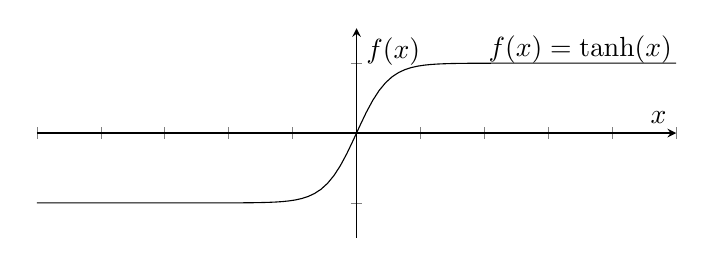
\begin{tikzpicture}
						\begin{axis}[
							xlabel = $x$,
							ylabel = {$f(x)$},
							xmin = -10, xmax = 10,
							ymin = -1.5, ymax = 1.5,
							width = 0.8\textwidth,
							height = 0.35\textwidth,
							xticklabel = \empty,
							yticklabel = \empty,
							axis lines = middle,
							domain = -10:10,
							samples = 100,
							]
							\addplot[black] {tanh(x)};
							\node at (axis cs: 7, 1.2) {$f(x) = \tanh(x)$};
						\end{axis}
					\end{tikzpicture}
					\caption{Tangente hiperbólica}
					\label{fig:funcion_tanh}
				\end{figure}
				
				De nuevo, esta función no devuelve valores binarios, y que guarda cierta relación con la logística, pues esta tiene también forma de sigmoide, pero a diferencia que la logística, esta verifica que $f(-x) = -f(x)$ por lo que es preferible sobre esta, y también hace que al usarla en redes neuronales su entrenamiento converja más rápido. Además $f: \mathbb{R} \longrightarrow (-1, 1)$ y su expresión es
				$$
				f(x) = \tanh(x) = \frac{\text{senh}(x)}{\cosh(x)} = \frac{e^x - e^{-x}}{e^x + e^{-x}}, 
				$$
				y verifica una segunda propiedad muy útil, es solución de la ecuación diferencial
				$$
				\frac{df}{dx} = 1 - f^2(x). 
				$$
				
				\item \textbf{Función ReLU}
				
				\begin{figure}[H]
					\centering
					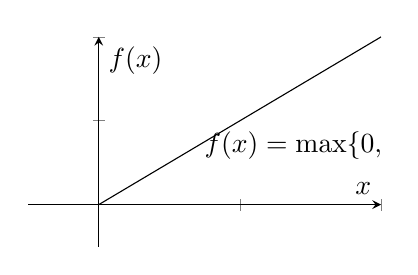
\begin{tikzpicture}
						\begin{axis}[
							xlabel = $x$,
							ylabel = {$f(x)$},
							xmin = -.5, xmax = 2,
							ymin = -.5, ymax = 2,
							width = 0.5\textwidth,
							height = 0.35\textwidth,
							xticklabel = \empty,
							yticklabel = \empty,
							axis lines = middle,
							domain = -.5:2,
							samples = 100,
							]
							\addplot[black, domain = 0:2] {x};
							\node at (axis cs: 1.5, .7) {$f(x) = \max\{0, x\}$};
						\end{axis}
					\end{tikzpicture}
					\caption{Función ReLU}
					\label{fig:funcion_relu}
				\end{figure}
				
				La función ReLU (Rectified Linear Unit) es una de las más populares al trabajar con redes neuronales, pues a pesar de que no es derivable en $x = 0$ (normalmente se soluciona tomando $f'(0) = 1$), soluciona un serio problema que causan las funciones logística y tangente hiperbólica durante el entrenamiento de una red neuronal. Este problema es conocido como \textit{vanishing gradient} y de forma resumida consiste en que cuando la derivada de una función de activación es muy próxima a cero, relentiza enormemente el proceso de aprendizaje, pues si se observa con detalle cómo se calculan las actualizaciones de los pesos y sesgos en el \Cref{algo:backprop}, si los términos $\delta^{(s)}$ tienden a cero, la diferencia entre los parámetros de una iteración a otra tiende a cero, necesitando una cantidad enorme de iteraciones. Como se observa a continuación, la función ReLU soluciona este problema. Además, la derivada es mucho más sencilla de calcular. 
				
				\begin{align*}
					\lim_{x\to\infty}\frac{d}{dx}\frac{1}{1+e^{-x}} = 0 && \lim_{x\to\infty}\frac{d}{dx}\tanh(x) = 0 && \lim_{x\to\infty}\frac{d}{dx}\text{ReLU}(x) = 1
				\end{align*}
				
				Si bien soluciona este problema mencionado para valores de $x > 0$, genera el mismo problema para valores negativos. Para solucionar este problema se suelen tomar variantes de la función ReLU conocidas como LReLU, PReLU, o ELU; que modifican su expresión para valores de $x \leq 0$ como funciones lineales o exponenciales. 
				
			\end{itemize}
			
		\section{Redes neuronales convolucionales}
		
			Una vez explicado cómo funciona una red neuronal y cómo puede usarse para problemas de regresión y clasificación, es interesante poder aplicar estas tareas sobre imágenes en vez de sobre conjuntos de datos numéricos. Una imagen de $n \times m$ píxeles en escala de grises puede entenderse como una matriz de $n \times m$ elementos, sin embargo, suelen utilizarse imágenes a color y esto se puede conseguir utilizando tres canales, rojo, azul, y verde. De esta forma, una imagen se representa como tres matrices. Formalmente, una imagen se representa como un tensor, que puede entenderse como un vector de matrices, o una estructura que indexa elementos mediante una tupla $(i, j, k)$\cite{introCNN}.\\
			
			De manera ingenua, una primera aproximación para clasificar imágenes en función de objetos que aparezcan en estas, podría ser linealizar este tensor y pasarlo como vector de entrada a un red neuronal multicapa, obteniendo un vector de salida que indique a qué clase pertenece la imagen. Esto, además de que no da resultados positivos, pues se da la misma importancia a todos los píxeles y se obvian detalles y características de la imagen, computacionalmente es muy complicado de abarcar. Suponiendo que se tiene una imagen RGB cuadrada de $n \times n$ píxeles, y que la primera capa oculta tuviera $m$ neuronas, el número de parámetros de esta capa sería $m(3n^2 + 1)$. Suponiendo imágenes de baja calidad, por ejemplo $64 \times 64$ píxeles, y que el número de neuronas de la primera capa fuese 5, el número de parámetros es de 61445. Ajustar adecuadamente esa cantidad de parámetros muy costoso, y además daría resultados muy pobres en el caso de encontrar los parámetros adecuados. 
 		
		
	
	\paginavacia
	\addcontentsline{toc}{chapter}{Bibliografía}
	\printbibliography
	
	% CONTRAPORTADA
	\chapter*{}
	\thispagestyle{empty}
	\cleartoleftpage
	\thispagestyle{empty}
	\BgThispage
	
	\begin{tikzpicture}[remember picture,overlay]
		\node[yshift = -5cm] at (current page.north west){
			\begin{tikzpicture}[remember picture, overlay]
				\draw[fill = headingPortadaTFG, headingPortadaTFG] (0,0) rectangle (\paperwidth,5cm);
				\node[yshift = 3cm, xshift = 0.5\paperwidth, font = \Huge, text centered, midway] {\color{textoHeadingPortadaTFG}\universidad};
				\node[yshift = 2cm, xshift = 0.5\paperwidth, font = \Huge, text centered, midway] {\color{textoHeadingPortadaTFG}\escuela};
			\end{tikzpicture}
		};
	\end{tikzpicture}
	
	\large
	\vspace{19.3cm}
	
	\begin{center}
		\centerline{
			
\includegraphics[height=2.5cm]{01_logo-vA_pant293.pdf}
		}
	\end{center}
	
\end{document}